\chapter{Introduction\label{cha:chapter1}}

The World Wide Web (W3) is a wide-area hypermedia information retrieval initiative aiming to give universal access to a large universe of documents \cite{www}.
\\
The Web works thanks to a set of standards and protocols that guarantee interoperability at various levels. 
It is designed for human interaction, but the next generation web aims to make the Web understandable by machines: The Semantic Web \cite{sematicWeb}.
\\
\\
As described in *Scientific American*, 
\textit{'The Semantic Web is an extension of the current web in which information is given well-defined meaning, better enabling computers and people to work in cooperation''} \cite{bernerslee2001semantic}.
\\
\\
The Hyper Text Markup Language (HTML) is the standard markup language used for structuring and displaying documents on the Web.
While this language is great for human users, it is not optimized for structure data processing \cite{herman2003semanticweb}. 
\\
Consider the following Airline Scraper example:
\begin{lstlisting}[language=HTML, caption={Example of HTML flight data from an Airline company}, label={lst:html-example}]
  <div class="flight-result">
      <h2>Berlin to New York</h2>
      <p>Airline: Lufthansa</p>
      <p>Price: $450</p>
      <p>Departure: 10:00 AM</p>
  </div>
  \end{lstlisting}
In this scenario, the labels of fields like "Price", "Departure", etc., are not standardized. If the Airline changes any of those labels, the data extractor algorithm breaks. 
Developers would need to monitor every single Airline website and update the data extractor algorithm as soon as possible in order to guarantee the availability of their scraping service \cite{herman2003semanticweb}.
\\
\\
It is now clear why the Semantic Web needs its own standard to describe web resources that need to be process by machines.
\\
\\
The Resource Description Framework (RDF) is a standard model for data exchange on the Web. It has features that facilitate the merging of data with different schemas, and it supports the evolution of schemas over time without requiring all the data consumers to be changed \cite{rdf}.
\\
RDF enhances the linking structure of the Web to use URIs to label both the relationships between entities and the entities themselves (aka “triple”). This model allows for structured and semi-structured data to be mixed, exposed, and shared among different applications.
This linking structure forms a directed, labeled graph, where the edges represent the named link between two resources, represented by the graph nodes. This graph view provides an accessible mental model for understanding RDF and it's often used with its visual explanations
\begin{figure}[htb]
  \centering
  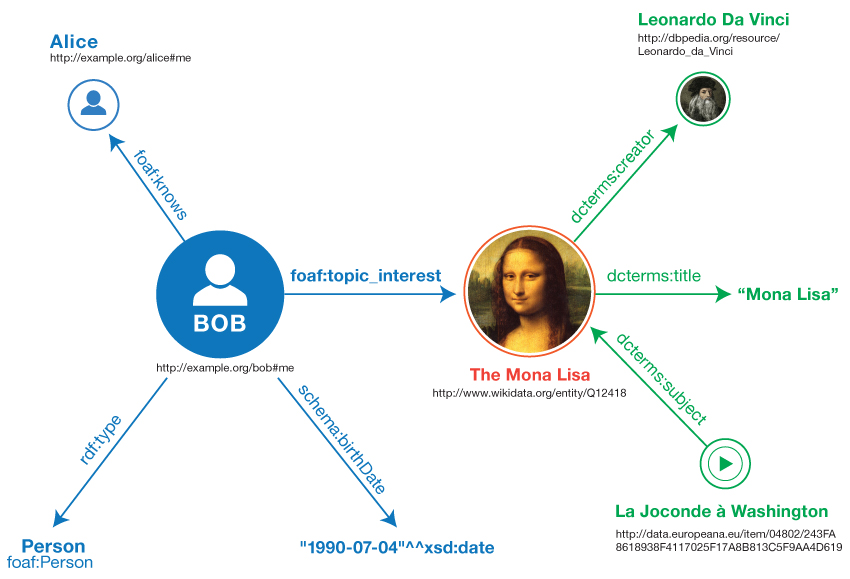
\includegraphics[width=15cm]{rdf-visual-representation-example.jpg}\\
  \caption{Example of RDF Graph}\label{fig:RDFTriple}
\end{figure}

Consider the following Airline Scraper RDF example:
\begin{lstlisting}[language=XML, caption={RDF representation of the flight data}, label={lst:rdf-example}]
  @prefix schema: <https://schema.org/> .
  
  <https://example.com/flights/12345> a schema:Flight;
      schema:departureAirport "Berlin" ;
      schema:arrivalAirport "New York" ;
      schema:airline "Lufthansa" ;
      schema:price "450"^^xsd:decimal ;
      schema:departureTime "10:00 AM"^^xsd:time .
  \end{lstlisting}
  In this scenario scenario, the Airline company has decided to adopt the RDF standard to describe their data.
  Developers can now query the Airline web service without worrying about breaks due to changes in the Airline company \cite{herman2003semanticweb}. 
\\
\\
The RDF standard is not exclusively used by web developers. It is also widely utilized by scientists, engineers, and researchers across various disciplines:
\begin{itemize}
  \item \textbf{Data Scientists}:
  \begin{itemize}
      \item RDF aligns with their work on structured data, semantic queries, and knowledge graphs.
      \item They use RDF to model relationships, extract insights from interconnected datasets, and support machine learning on graph data.
  \end{itemize}
  
  \item \textbf{Computer Scientists and Engineers}:
  \begin{itemize}
      \item They focus on RDF’s theoretical foundations, optimization of storage and querying, and application development for the Semantic Web.
      \item They are often involved in creating RDF tools like RDF stores and query languages.
  \end{itemize}
  
  \item \textbf{Knowledge Engineers}:
  \begin{itemize}
      \item Specialize in designing ontologies and frameworks using RDF to represent knowledge in areas like AI, natural language processing, and expert systems.
  \end{itemize}
\end{itemize}

To assist Scientists in their work, the Semantic Web supports a set of tools and technologies that enable the creation, sharing, and analysis of structured data.
Platforms like Protégé, Apollo, and NeOn are well-known in the ontology engineering community. 

"An Ontology is a knowledge structure used to formally represent and share domain knowledge through the modeling and creation of a framework of relevant concepts and the semantic relationships between the concepts" \cite{ontology}.

These ontology editors offer comprehensive support for creating and editing ontologies and RDF datasets through their graphical user interfaces (GUIs), which enhance visualization and make RDF development easier.

\section{Motivation Scenario\label{sec:moti}}

The following hypothetical scenario illustrates the current situation.
\\
John Doe is a Junior Software Developer and just started working in his first company as Web Developer.
He quickly immersed himself in his daily tasks, working with his favorite IDE, Visual Studio Code, to craft the backbone of their innovative web application—a platform with social media-like features. 
\\
\\
While John primarily worked with VSCode due to its lightweight and customizable nature, he soon realized that his workflow differed significantly from that of his colleagues. Some teammates preferred IntelliJ IDEA for its extensive refactoring tools, while others relied on Protégé because its visual representation of ontologies helped them better understand and manage complex data relationships.
\\
\\
A significant part of the project involved working with RDF files, mainly RDF/XML and Turtle formats, to define the application's semantic data structure and its RDF schema. Although the project repository already contained some instances examples, John found himself losing a lot of time creating a valuable amount of example instances to test the limitation of his RDF schema. This extra step, required to ensure that every modification produced the intended results, often disrupted his coding flow.
\\
\\
Although he is writing in Turtle language for the majority of his time and Turtle is the most readable among all the RDF formats, John also struggles to read and understand many lines of code and often mistake like every other human being. Just like his colleagues, he started using an RDF schema visualizer like "isSemantic.net" or RDF Grapher, to see a graphical representation of his RDF schema \cite{issemantic,rdfGrapher}. The representation helps him a lot to identify relations errors, but importing his schema in another software every time contributes to the interruption of his workflow.


\section{Theses and Scientific Contribution  \label{sec:objective}}
The previous scenario highlights two big challenges. The first is the lack of a seamless integration between specialized development environments and RDF visualization tools. 
Developers should be free to choose the IDE that best suits them, but the disjointed process of visualizing semantic data remains a critical bottleneck.
\\
\\
The second challenge lies in the inefficiency of testing and validating RDF schemas. Manually generating new instances to test schema's limitations remains a major time-consuming task. Developers must invest considerable effort in creating and maintaining test data, moving their focus from core development activities. This repetitive manual work not only delays progress but also increases the risk of inconsistencies and undetected schema flaws.
\\
\\
This Master's Thesis aims to address these challenges and tries to incorporate all developer tools into a single environment.
By developing an IDE extension, developers will be able to handle RDF writing, data visualization, and instance generation in one place.
This IDE extension could support the direct editing of the generated instances, allowing for a more streamlined and efficient workflow.


\section{Positioning within the Scientific Context \label{sec:scope}}
This Thesis is positioned in the domain of Semantic Web and RDFs. It tries to address in the integration of development environments, RDF visualization and RDF instances generation, to enhance both theoretical understanding and practical application in the field.
\\
\\
As stated in the previous sections, the Semantic Web and RDFs, are very important for the scientific community. Their goal is to simplify machines' and computer scientists' lives when extracting and processing a vast amount of information from the W3.
Despite all its advantages, the Semantic Web struggles to move beyond academic use and find widespread commercial applications. 
There is indeed a lack of tools that can help engineers to work with RDFs and the Semantic Web to facilitate the creation and management of RDF Data. 
Among the most popular Integrated Development Environments, like Visual Studio Code, IntelliJ IDEA, and others, we can mainly find extensions that support syntax highlighting, with grammar checker and SHACL validators, and only one VSCode extension for the visualization of RDFs limited to the N3 and Turtle formats \cite{vscode_rdf_plugin,jetbrains_rdf_plugin,stackoverflow_survey_2024} (see Figure~\ref{fig:RDF-term-in-vscode-marketplace}).
\begin{figure}[htb]
  \centering
  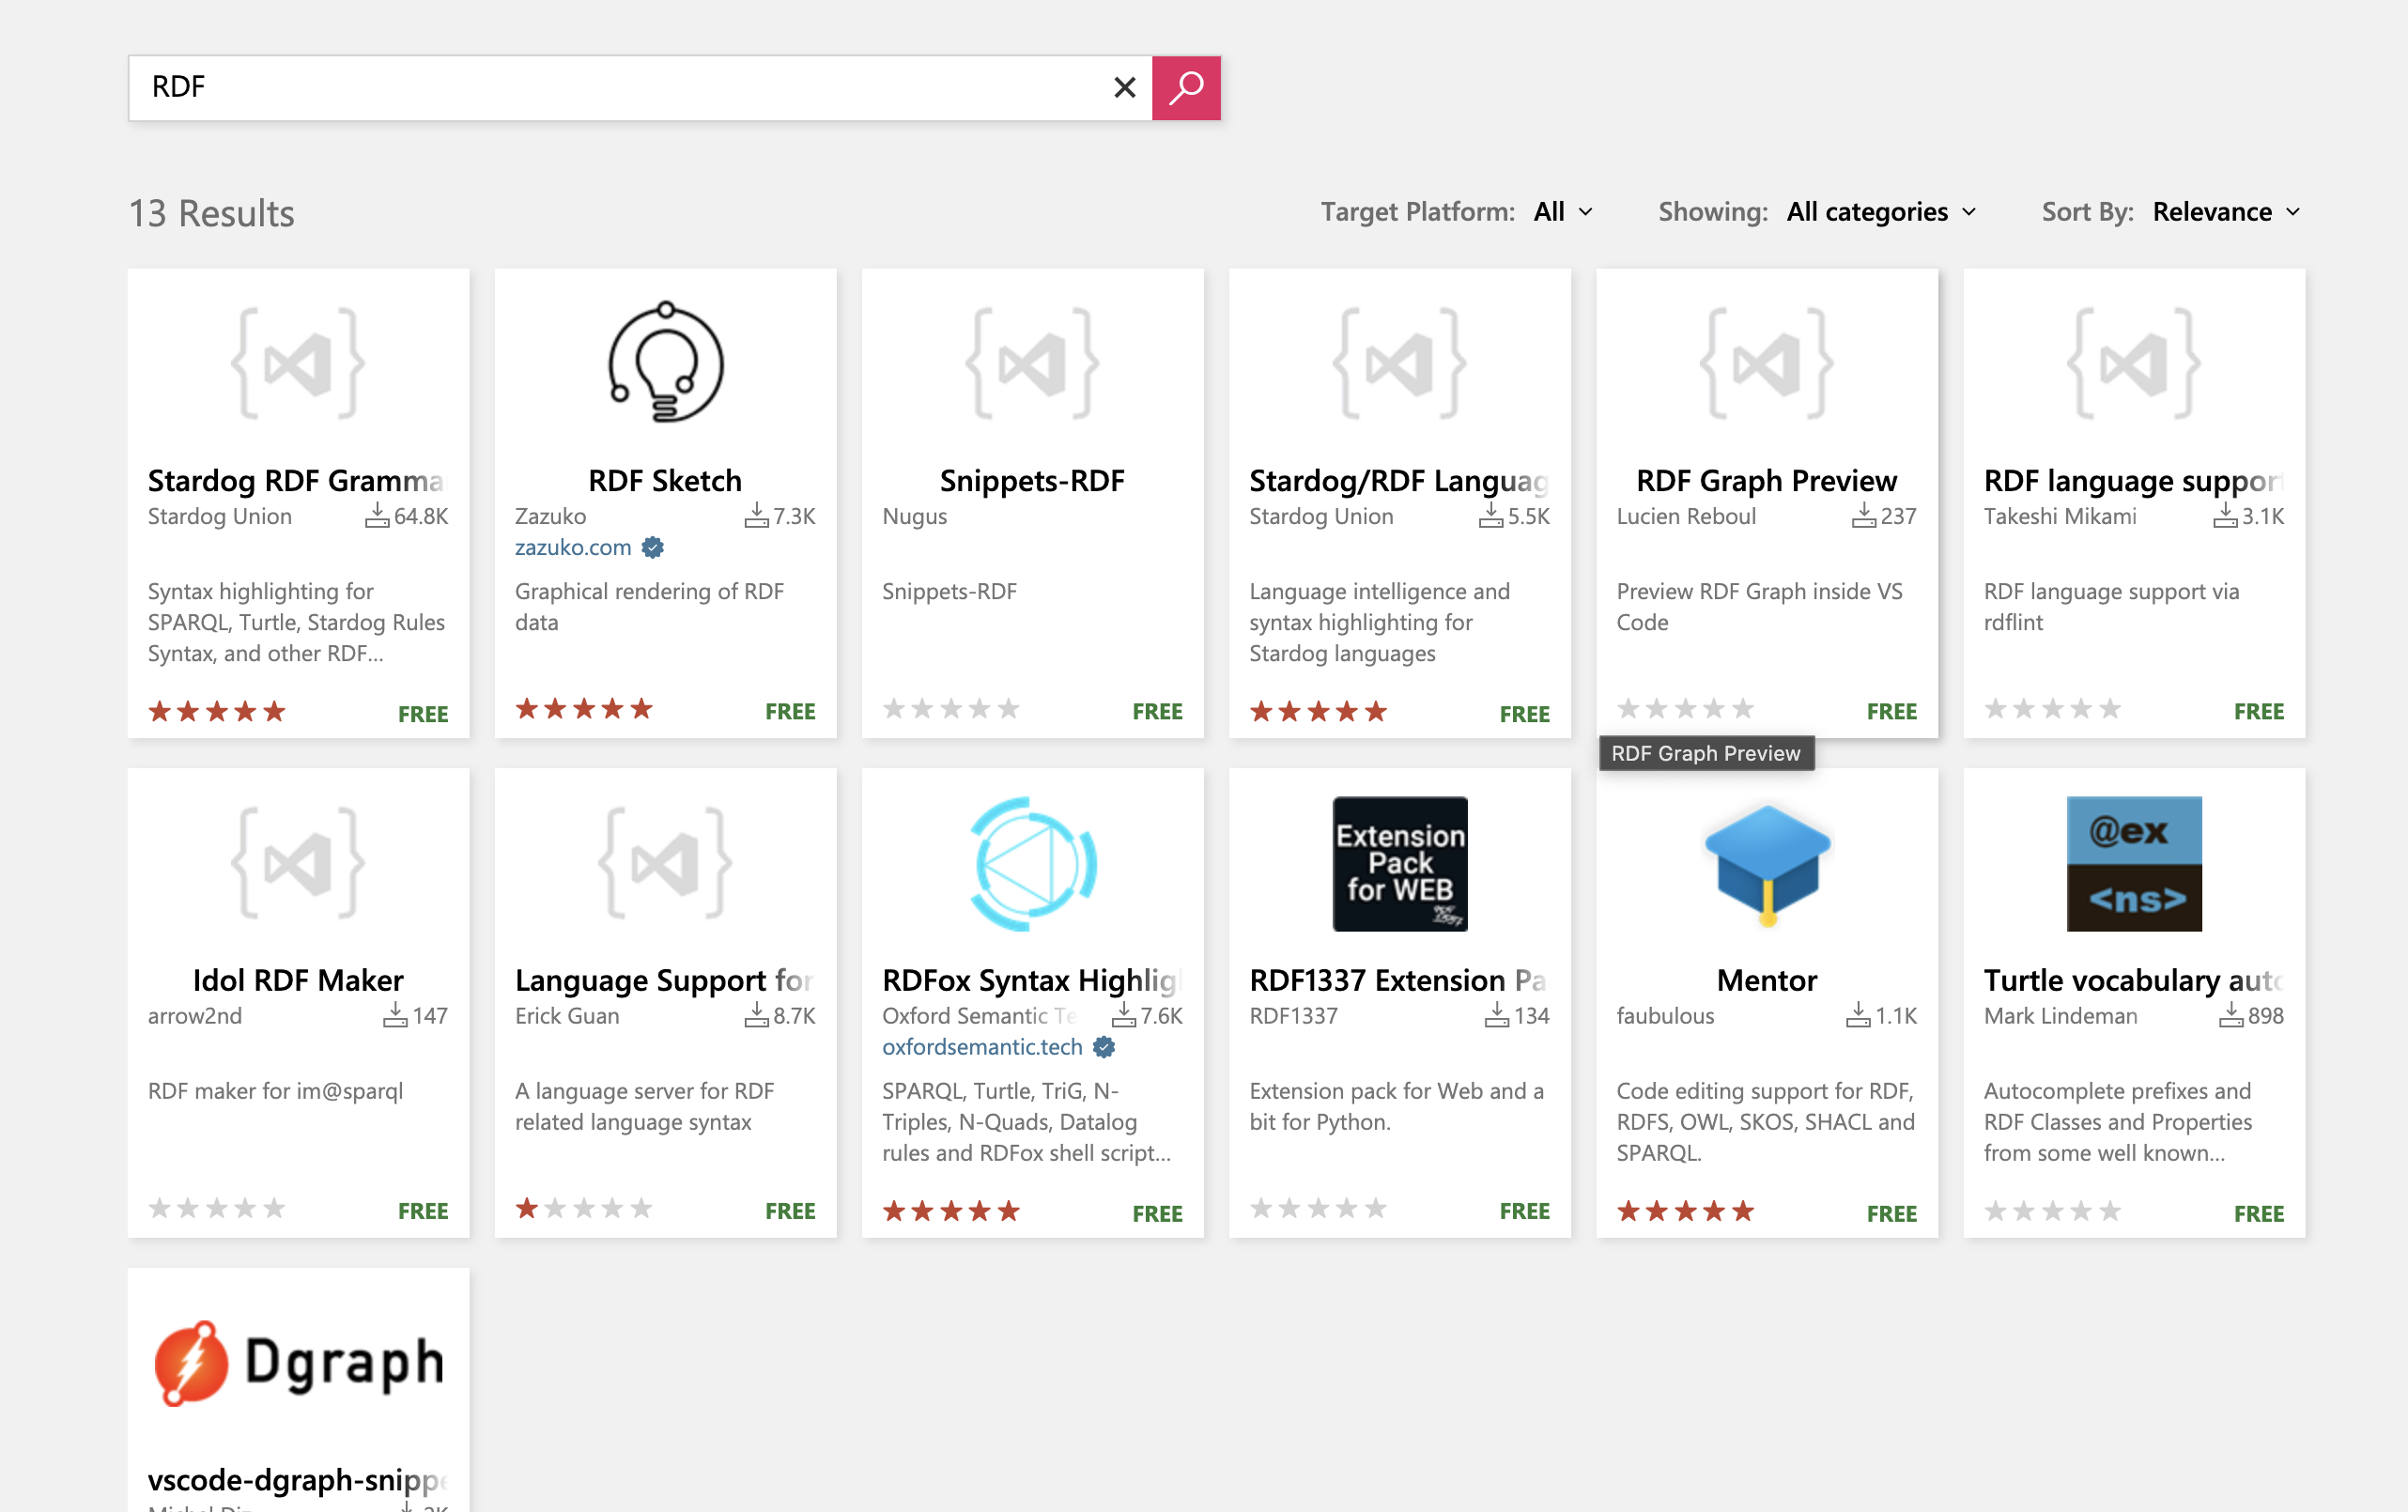
\includegraphics[width=13cm]{RDF-term-in-vscode-marketplace.png}\\
  \caption{Limited Support: A Search for 'RDF' in the Plugin Marketplace Yields Only 13 Results, Highlighting the Scarcity of RDF-Specific Extensions for Developers.}\label{fig:RDF-term-in-vscode-marketplace}
\end{figure}
\\
\\
The Semantic Web community needs a solution that could bridge this gap, something that is not limited to a specific software, architecture, or environment. A solution that could potentially be compatible with every IDE and Browser. An open-source software with and MIT license can be enhanced not just by the community, but also by companies and institutions.
A program with a core that allows an easy integration of modules and plugins. 
\\
\\
For this Master's Thesis, I will develop a Web Service using Python 3.11 and the Fastapi library, able to process the most common RDF formats, generate n amount of instances for a given RDF Schema, and return the desired results. 
The outcome will be provided in different formats, but mainly served as HTML pages, so that can be processed by a Visual Studio Code extension in a Web View. This approach will limit the service to be used only by the VSCode IDE, but by all the ones that support rendering of HTML content in their environment.
\\
\\
To prove the validity of this approach, I will develop not just the Visual Studio Code extension using TypeScript, but also a dedicated browser frontend view, and an IntelliJ IDEA plug-in, in Kotlin, with a limited set of features. 
These Client Side applications will communicate with the Web Service, and via REST calls. The user will be able to: 
\begin{itemize}
      \item Send an RDF Schema to the Web Service
      \item Request an n amount of instances for the given schema
      \item Edit the RDF Schema with the instances generated by the server
      \item Visualize the RDF
      \item Download the Graph as an image. 
\end{itemize}
% limitations
Due to the vastness of this project, some features will only be deepened in a theoretical manner, like the AI Instance Generation, and only some because features for the IntelliJ IDEA plugin will be covered.
\\
\begin{figure}[htb]
  \centering
  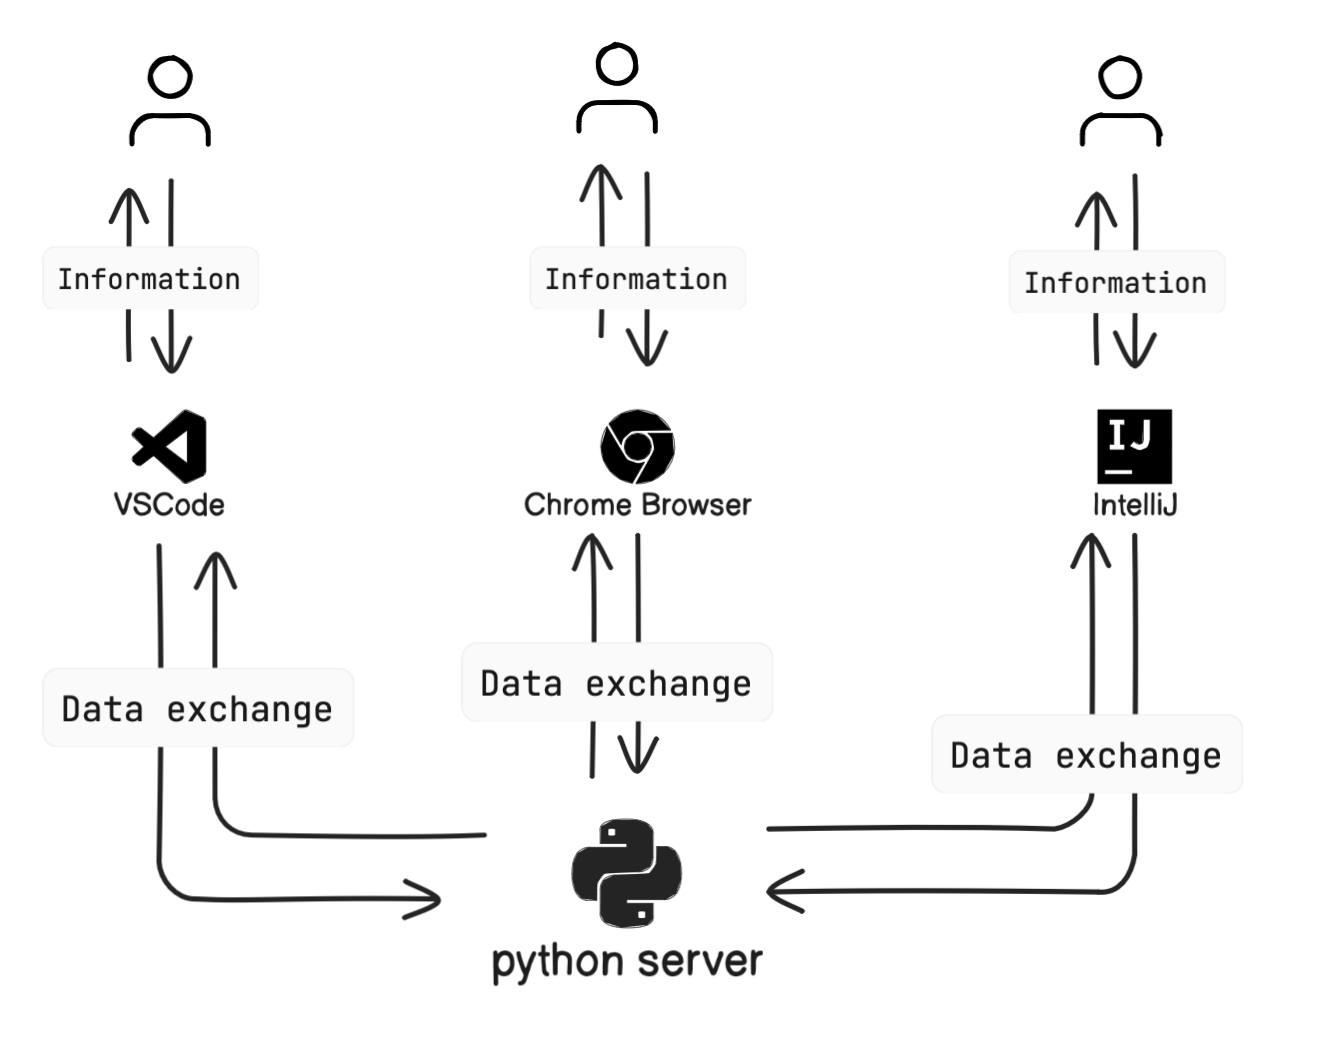
\includegraphics[width=13cm]{schema_architecture_1_white.png}\\
  \caption{System Architecture: Information Flow and Data Exchange between Users, Development Environments (VSCode, IntelliJ), Chrome Browser, and a Python Server.}\label{fig:intro}
\end{figure}

\section{Structure of the Work \label{sec:outline}}

This thesis is separated into 7 chapters.
\\
\\
\textbf{Chapter \ref{cha:chapter2}: State of the Art} covers the related work in the RDF world, from the instance generation to the graph visualization. 
\\
A short view of existing tools and projects in the same domain, like GAIA and Ontodia.
\\
A comparison of the two different approaches in terms of instance creation (Manual vs Automatic).
% in this actually you should talk a lot about A-BOX and T-Box
A brief look at the current standards and technologies compatible with the semantic Web and RDFs.
\\
\\
\textbf{Chapter \ref{cha:chapter3}: Concept} includes the requirements for the project, a view of the technologies and high-level architecture, and the constraints and goals of this work.
\\
\\
\textbf{Chapter \ref{cha:chapter4}: Implementation} features the implementation of the project with all its components. Describe in very detail the design choices, building blocks, and algorithms of this system.
\\
\\
\textbf{Chapter \ref{cha:chapter5}: Evaluation} explains how the implementation is validated. Portrays benchmarks and measurements regarding the performance of the solution. Showcases some examples of RDF generation and graph visualization. Cite the experience of a group of Computer Scientists. 
\\
\\
\textbf{Chapter \ref{cha:chapter6}: Conclusion and Limitations} summarizes the thesis, describes the problems that occurred. 
\\
\\
\textbf{Chapter \ref{cha:chapter7}: Outlook} Discusses the future of the project, and the possible improvements that can be done, like the integration of an AI model and the support for further ontologies.